\documentclass{article}
\usepackage{url}
\usepackage{natbib}
\usepackage{float}
\usepackage{graphicx}
\usepackage{nextpage}
\pagestyle{headings}
\setcounter{tocdepth}{1}
\setlength{\voffset}{-1.5cm}
\setlength{\hoffset}{-2.5cm} \setlength{\textwidth}{16.5cm}
\setlength{\textheight}{23cm}
\title{Pacific Rock Art}
\author{John Maindonald, using resources supplied by Meredith Wilson}
\begin{document}
\maketitle
\paragraph{Dataset \texttt{rockArt} -- List of Motifs}

\begin{verbatim}
Circle (C) 
Ca1  (1)
Ca2 Ca3 Ca4[9] Cb5 Cb6 Cc7  (2)
Cc8 Cc9 Cc10 Cc11 Cc12 Cc13 Cc14 Cc15 Cc16 Cc17 Cc18 Cc19
Cc20 Cd21  (3)
Cd22 Cd23 Cd24 Cd25[10] Cd26[10] Cd27[1] Ce28 (4)
Ce29 Cf30 Cf31 Cf32 Cf33 Cf34 Cf35 Cf36 Cf37 Cf38 Cg39 (5)
Cg40 Ch41 (6)
Ch42 Ci43  (7)
Ci44 Cj45  (8)
Ck46  (9)
Ck47 Cl48  (10)
Cm49 Cm50 Cm51 Cm52 Cm53 Cm54 Cm55 Cm56 Cm57 Cm58 Cn59  (11)
Cn60 Cn61 Cn62 Cn63 Cn64 Cn65 Cn66 Cn67 Cn68 Cn69 Cn70 Cn71 Co72  (12)
Co73 Co74 Co75 Co76 Co77 Co78 Co79 Cp80 Cq81 (13)
Cq82 Cq83 Cq84 Cq85 Cq86 Cq87 Cq89 Cq90
Cq91 Cq92 Cq93 Cq94 Cq95 Cq96 Cq97 Cr98 (14)
Cr99 Cr100 Cr101 Cs102  (15)
Cs103 Cs104 Cs105 Cs106 Ct107 Cu108  (16)
Cv109  (17)
Cw110  (18)
Cx111  (19)

Semi-circle (SS) 
SSa1  (20)
SSd2 SSd3 SSd4 SSd5 SSd6 SSd7
SSe8  (21)
SSf9 SSg10  (22)
SSj11  (23)
SSj12 SSj13  (24)
SSl14  (25)
SSm15 SSm16 SSn17 (26)
SSn18 SSn19 SSn20 SSn21 SSn22 SSn23 SSn24 SSn25 SSn26 SSn27
SSn28 SSn29 SSn30 SSu31  SSu32 SSn33 SSn34 SSn35 SSo36 SSo37  (27)
SSp38[26] SSq39 (28)
SSq40 SSt41 (29)
SSu42 (30)

Oval (O) 
Oa1  (31)
Oa2[32] Od3 Od4 Oe5  (32)
Of6 Of7 Of8 Og9  (33)
Og10  (34)
Og11 Og12 Og13 Og14
Oj15 Oi16  (35)
Om17  (36)
Om18 Om19 Om20 Om21 On22  (37)
On23 On24 Oq25[36] Oq26[37] Oq27[36] Ou29[34] Ov30[37] Ov31[36] O32(38/39) O33  (40)
O34[37] 

Spiral (S)
Sa1  (41)
Sb2 Sb3 Sd4 Sd5 Sd6 Sd7 Se8 Si9 Sm10 Sm11 S12 S13 Sx14 Sx15 Sx16 Sx17 
Sy18 Sz19 S20 S21 S22 S23 S24 S25 
Scroll (SC) 
SCd1  (42)
SCd2 SCd3 SCd4 SCd5 SCd6 SCd7 SCd8 SCn9 SCn10 SCw11 SCx12 SCx13 SCx14 SCx15 
SCx16 SCy17 SCy18 SC19 SC20 SC21 SC22 SC23 SC24 SC25 SC26 
Star-shaped (SR) 
SRd1  (43)
SRd2 SRd3 SRd4 SRf5 SRf6 SRf7 SRj8 SR9 SR10 

Bean-shaped (B) Bd1  (44)
Bn2 Bn3 Bn4 Bt5 Bx6 

Heart-shaped (H) 
Ha1  (45)
Hg2 Hn3 Hq4 Hq5 

Teardrop-shaped (TD) TDd1  (46)
TDf2 TDj3 TDn4 TDq5  (47)
TD6 TD7 TD8 TD9 

Diamond (D) Dc1  (48)
Dg2 Dh3 Dk4 Dm5 Dm6 D7 

Diamond (D) D8 D9 D10 D11 D12 D13 

Triangle (T) Ta1  (49)
Tc2 Tc3 Tc4 Td5 Tf6 Tf7 Tg8 Th9 To10 T11 T12 T13 T14 T15 T16 

Conical (CN)
CNg1  (50)
CN2 CN3 CN4 CN5 CN6 CN7 CN8 

Leaf-shaped (L) Ld1  (51)
Lf2 Lg3 Lp4 L5 L6 L7 L8 L9 L10 L11

(L)-stencil  (LS)  
LS1[105] LS2[105] 

(L)-with linear ext. (LL)  LL1  (52)
LL2 LL3 LL4 LL5  

Ovoid (EG)
EGd1  (53)
EGf2 Curved conical (CC) CCd1  (54)
CCn2 CCn3 Closed 'M' (EM) EMc1  (55)
EMd2 EMd3 EMf4 EMf5 EMn6 EMx7 EM8 EM9 EM10 EM11 EM12  

(TD) with extensions (TE)
TE1  (56)
TE2 TE3 TE4 TE5 

Bow-shaped (BW) 
BWe1  (57) BWn2 BWn3 

Toadstool-shaped (TS)
TS1  (58)
TS2 TS3 TS4 TS5 TS6 TS7 TS8 TS9 

Paddle-shaped (P) 
Pg1  (59)
Pg2 Pg3 

Double 'u' (DU) 
DUaa1 (60)
DUw2 DU3 

Cupule/dot (CP) 
CP1  (61)
CP2 CP3 CP4 CP5 CP6 CP7 CP8 CP9 CP10 CP11 CP12 

"Straight" line (ST) STd1  (62)
STd2 STd3 STg4 STaa5 STaa6 STaa7 STaa8 ST9  (63)
ST10 ST11  (64)
STd12 Wavy line (W) Wd1  (66)
Wd2 Wd3 Wd4 Wn5 Waa6 Waa7 W8 W9 W10 W11 W12 W13 

Zig-zag (Z) Zd1  (67)
Zd2 Zn3 Zw4 Zw5 Zaa6 Z7 Z8 Z9 Z10 Z11 Z12 

Central line (CL) 
CLd1  (68)
CLd2 CLd3 CLd4 CLd5 CLd6 CLd7 CLd8 CLd9 CLd10 CLd11  (69)
CLd12 CLd13 CLd14 CLd15 CLd16 CLd17 CLd18 CLd19 CLd20 CLd21[68] 
CLd22[68] CLd23 (70)
CLd24 (71)
CLd25[68] CLd26 (72)
CLd27 CLd28
CLd29 CLd30 CLd31 (73)
CLd32 CLd33 CLd34 (74)
CLd35 (75)
CLd36 (76)
CLd37 (77)
CLd38 (78)
CLn39 (79)
CLn40 CLn41 CLn42 CLn43 CLn44 CLn45 CLn46 CLn47 CLn48 CLw49 (80)
CL50 CL51 CL52 (81)
CL53 CL54 CL55 CL56 (82)
CL57[79]
CL58 (83)
CL59[68] 

Cross (X) Xd1  (84)
Xd2 Xd3 Xd4 Xd5 Xd6 Xd7 Xd8 Xd9 Xd10 Xd11  (85)
Xd12[84] Xd13 Xf14[84] Xk15 Xn16  (86)
Xn17 Xn18 Xn19 Xn20 Xn21 Xn22 Xn23 Xn24 Xn25 Xn26 Xn27 Xn28 Xn29 Xn30 
Xn31 Xn32 Xp33 Xp34 Xp35 Xq36 Xq37 Xq38 X39[84] X40[85] X41  (87)
X42  (88)
X43[86] X44[84] X45  (89)
X46  (90)
X47[84]
X48[84] X49  (91)
X50 

Quadrilateral (Q) 
Qd1  (92)
Qe2 Qe3 Qh4 Qh5 Qh6 Qh7 Qh8 Qh9 Qn10 Qn11 Qt12 Q13 Q14 Q15 Q16
Q17 Q18 Q19 Q20 Q21 Q22 Trapeze (TZ) TZd1  (93)
TZf2 TZh3 TZ4 

Concave rectilinear (CR) 
CRd1  (94)
CR2 CR3 

Elongated u-shape (EU) 
EUd1  (95)
EUd2 EUg3 EUm4 EUw5 EU6 

U-shaped (U) 
Ud1  (96)
Ud2 Ud3 Uaa4 U5 

V-shaped (V)
Va1  (97)
V2 V3 V4 V5 

Line w/extensions (LWE) 
LWE1  (98)
LWE2 

Arc (A) 
Ad1  (99)
Al2 Am3 An4 Aw5 Aaa6 A7 A8 A9 

Elongated v-shape (EV) 
EVd1 (100)
EVg2 

Tick (TK) T
K1 (101)

Elongated w/lines (ECL) 
ECL1 (102)

Elongated form (EF) 
EFe1 (103)
EFm2 EFm3 EF4

Lollipop-shaped (TR) 
TRo1 (104)
TRq2 TR3 TR4 TR5 

Petal-shaped (PT) 
PT1 (106)
\end{verbatim}

\paragraph{Examples of motifs}
\begin{figure}[h]
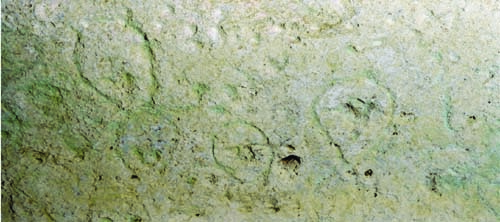
\includegraphics{plate12}
\caption{Examples of engraved 'eye-nose' faces, Apialo (MK15), Northwest 
Malakula}
\end{figure}
     


\begin{thebibliography}{99}
\bibitem[Wilson (2005a)]{Wilson05a} Wilson, M. 2005.
\emph{Picturing Pacific Pre-History} (PhD thesis), 
Australian National University.
\bibitem[Wilson (2005b)]{Wilson05b} Wilson, M. 2005.
Rethinking regional analyses of Western Pacific rock-art. 
\emph{Records of the Australian Museum}, Supplement 29: 173-186.
\end{thebibliography}

\end{document}





